\chapter{ATB Transmitter}\label{atb_transmitter}

The \textit{ATB Transmitter} module performs transactions using the AMBA ATB protocol.
This module is fundamental to make the TE communicate with the outside world.

\section{Signals necessary}
The AMBA ATB specification requires the following signals, grouped by usage.

\begin{table}[H]
    \centering 
    \begin{tabularx}{\textwidth}{|c|c|c|>{\centering\arraybackslash}X|}
        \hline
        Signal      & Transmitter   & Receiver  & Description \\ \hline
        ATCLK       & Input         & Input     & Global ATB clock. \\ \hline
        ATCLKEN     & Input         & Input     & Enable signal for ATCLK domain. This signal is 
                                                  optional.\\ \hline
        ATRESETn    & Input         & Input     & ATB interface reset, active LOW. This signal is 
                                                  asserted LOW asynchronously, and deasserted 
                                                  HIGH synchronously. \\ \hline
    \end{tabularx}
    \caption{ATB global signals} 
    \label{tab:global_signals}
\end{table}

\begin{table}[H]
    \centering 
    \begin{tabularx}{\textwidth}{|c|c|c|>{\centering\arraybackslash}X|}
        \hline
        Signal          & Transmitter   & Receiver  & Description \\ \hline
        ATBYTES[m:0]    & Output        & Input     & The number of bytes on ATDATA to be 
                                                      captured, minus 1. \\ \hline
        ATDATA[n:0]     & Output        & Input     & Trace data. \\ \hline
        ATID[6:0]       & Output        & Input     & An ID that uniquely identifies the source 
                                                      of the trace. \\ \hline
        ATREADY         & Input         & Output    & The Receiver is ready to accept data. \\ \hline
        ATVALID         & Output        & Input     & A transfer is valid during this cycle. If 
                                                      LOW, all other AT signals must be ignored. \\ \hline
    \end{tabularx}
    \caption{ATB data signals} 
    \label{tab:data_signals}
\end{table}

\begin{table}[H]
    \centering 
    \begin{tabularx}{\textwidth}{|c|c|c|>{\centering\arraybackslash}X|}
        \hline
        Signal  & Transmitter   & Receiver  & Description \\ \hline
        AFVALID & Input         & Output    & The flush signal to indicate that all buffers must 
                                              be flushed because trace capture is about to stop. \\ \hline
        AFREADY & Output        & Input     & The flush acknowledge to indicate that buffers have 
                                              been flushed. \\ \hline
    \end{tabularx}
    \caption{ATB flush control signals} 
    \label{tab:flush_control_signals}
\end{table}

\begin{table}[H]
    \centering 
    \begin{tabularx}{\textwidth}{|c|c|c|>{\centering\arraybackslash}X|}
        \hline
        Signal  & Transmitter   & Receiver  & Description \\ \hline
        SYNCREQ & Input         & Output    & The synchronization request signal to request the 
                                              insertion of synchronization information in the 
                                              trace stream. \\ \hline
    \end{tabularx}
    \caption{ATB synchronization request signals} 
    \label{tab:synchronization_signals}
\end{table}

\begin{table}[H]
    \centering 
    \begin{tabularx}{\textwidth}{|c|c|c|>{\centering\arraybackslash}X|}
        \hline
        Signal      & Transmitter   & Receiver  & Description \\ \hline
        ATWAKEUP    & Input         & Output    & The wake-up signal indicating any activity 
                                                  associated with an ATB interface. \\ \hline
    \end{tabularx}
    \caption{ATB wake-up signals} 
    \label{tab:wake-up_signals}
\end{table}

\section{Transactions}

The fundamental transactions that can happen are the following:
\begin{itemize}
    \item   Data transfer.
    \item   Flush control.
    \item   Synchronization.
\end{itemize}

This module can be instantiated to use different sized data bus, given they are compliant with 
the ones defined in the specification.

Within the AMBA ATB specification are defined different functionalities and some of them are 
optional. Here is a table that shows which are implemented and which are not:
\begin{table}[H]
    \centering
    \begin{tabular}{|c|c|} 
        \hline
        Feature         & Supported \\ \hline
        Flush control   & yes       \\ \hline
        Synchronization & no        \\ \hline
        Wake-up         & no        \\ \hline
    \end{tabular}
    \caption{ATB features supported by the ATB transmitter module} 
    \label{tab:ATB_supported_features}
\end{table}

\subsection{Data transfer}
\begin{figure}[H]
    \centering
    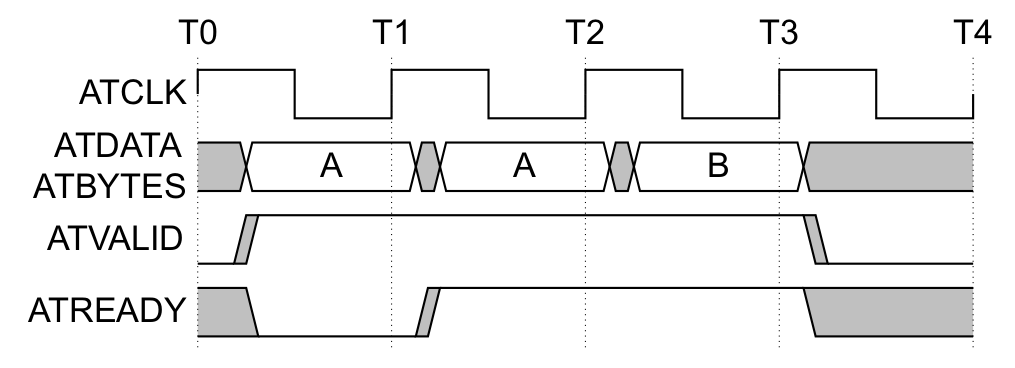
\includegraphics[width=0.8\textwidth]{img/atb_data_transfer.png}
    \caption{ATB data transfer}
    \label{fig:atb_data_transfer}
\end{figure}

The transfer is initiated by the transmitter that asserts the \texttt{ATVALID} signal and puts 
data along with the number of valid bytes (\texttt{ATBYTES}) on the bus. The \texttt{ATVALID} 
signal is asserted and data are kept on the bus until the receiver asserts the \texttt{ATREADY} 
signal, meaning the data can be read.

\section{Flush control}
The buffer flush is used to clean the FIFO to prepare for new data as cycles progress.
The handshake changes depending on the architecture used for the Transmitter: with or without 
internal storage.

\subsection{Transmitter with internal storage}
\begin{figure}[H]
    \centering
    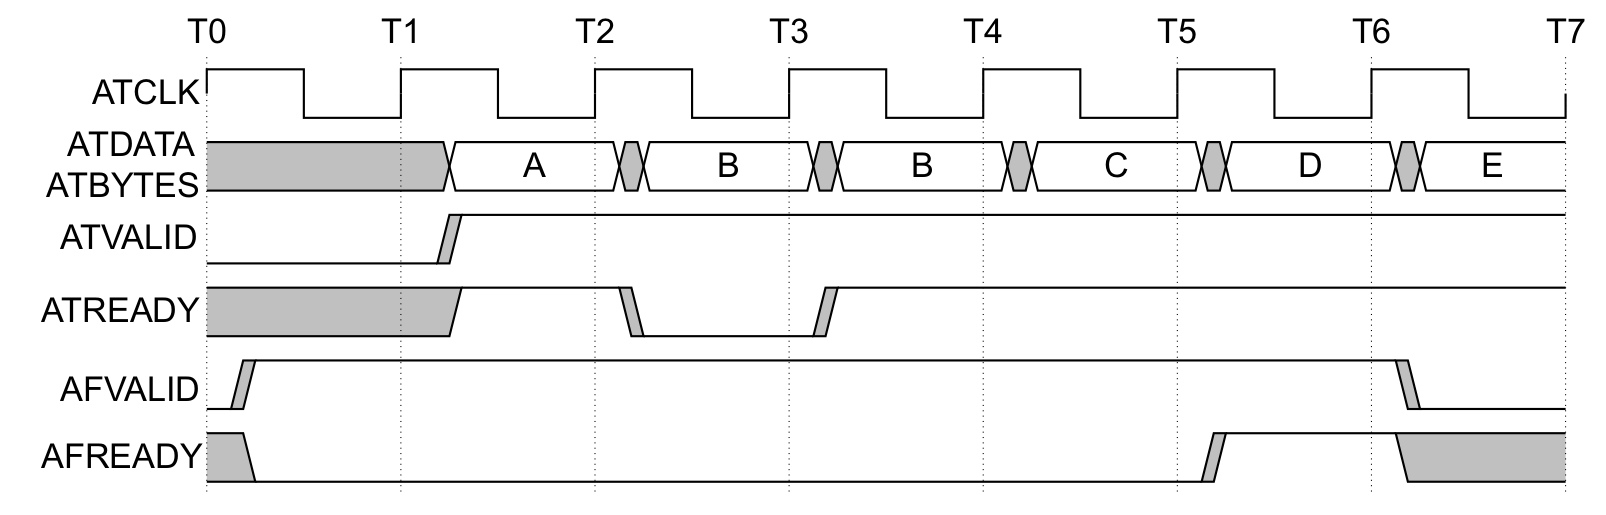
\includegraphics[width=0.8\textwidth]{img/atb_flush_store.png}
    \caption{ATB flush transmitter with storage}
    \label{fig:atb_flush_store}
\end{figure}

When the \texttt{AFVALID} signal coming from the receiver is asserted, the Transmitter starts 
outputting the data stored and generated until the \texttt{AFVALID} signal was received.
When all the data stored before the receiving of the \texttt{AFVALID} signal have been sent, 
the \texttt{AFREADY} signal is asserted. This signal does not mean the FIFO is empty.

\subsection{Transmitter with no internal storage}

\begin{figure}[H]
    \centering
    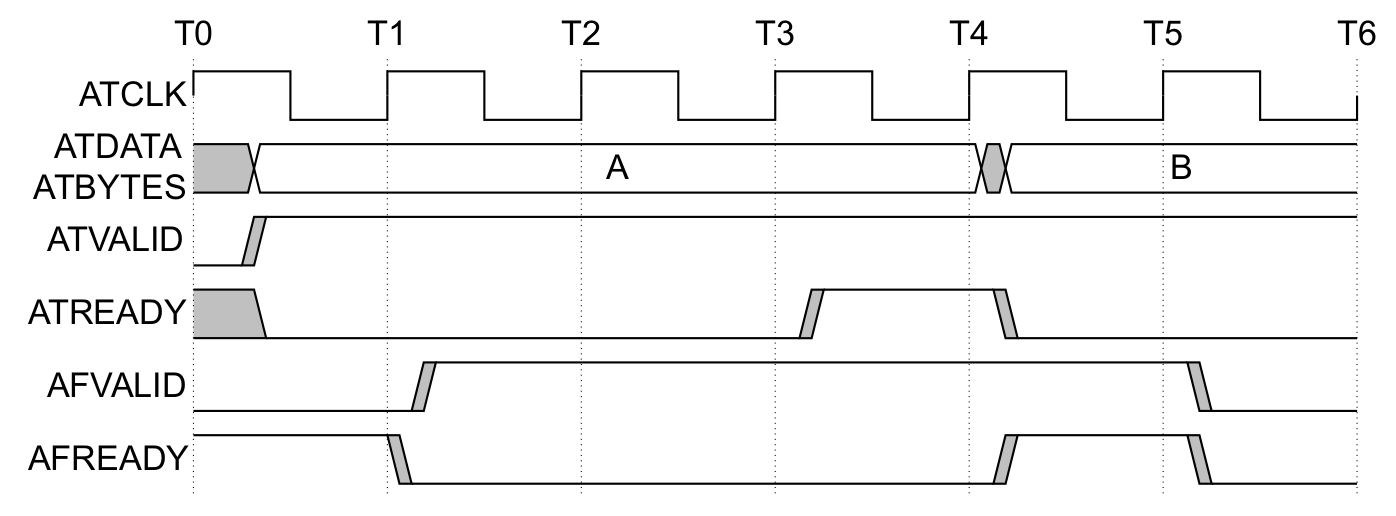
\includegraphics[width=0.8\textwidth]{img/atb_flush_no_store.png}
    \caption{ATB flush transmitter with no storage}
    \label{fig:atb_flush_no_store}
\end{figure}

In case the Transmitter has no internal storage, the flush can be done.
In this scenario, the packet considered "old" and to be flushed is the one that the Transmitter 
is trying to send when the \texttt{AFVALID} signal is received.
The cycle after the "old" packet has been sent, the \texttt{AFREADY} signal is asserted 
communicating to the Receiver the flush has been completed.

\begin{figure}[H]
    \centering
    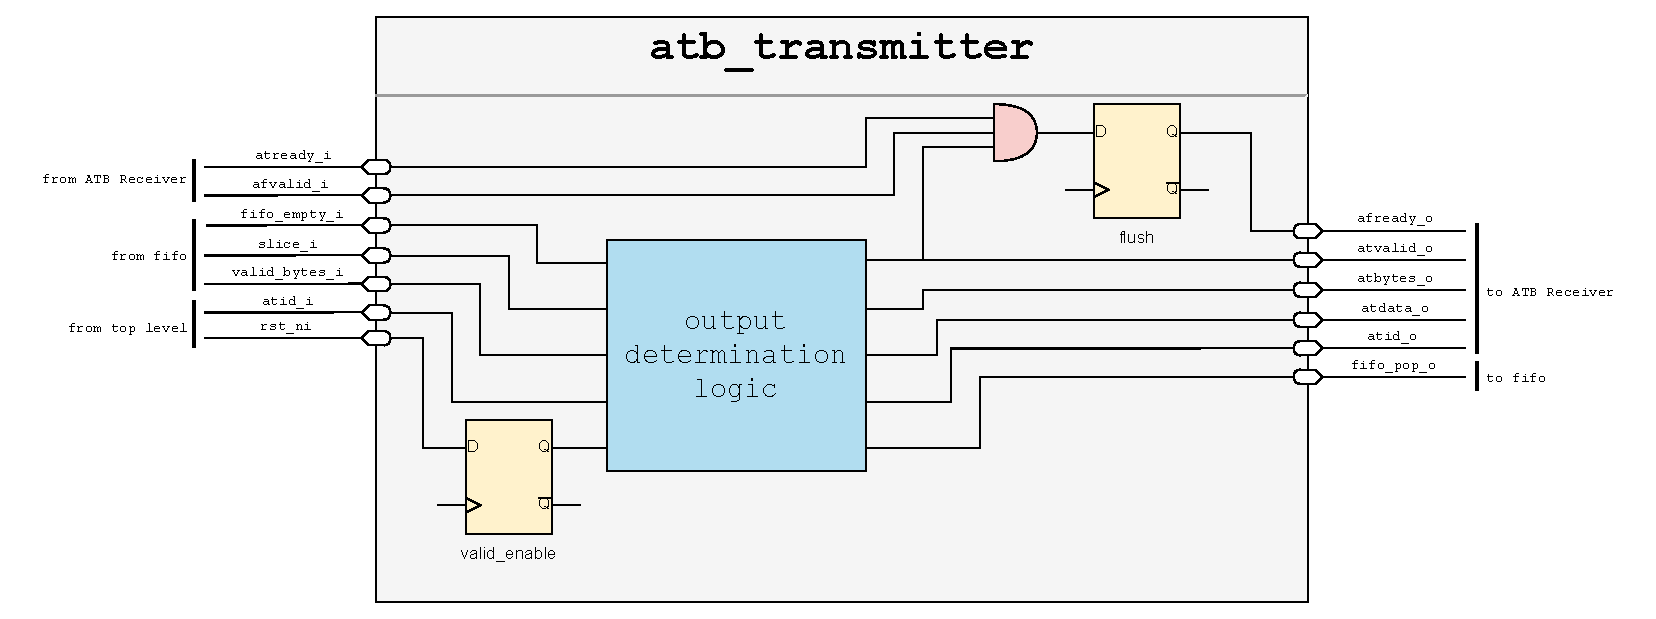
\includegraphics[width=1\textwidth]{img/atb_transmitter.pdf}
    \caption{ATB Transmitter module internal architecture}
    \label{fig:atb_transmitter_architecture}
\end{figure}